\pagestyle{empty}
\section{Client and visualisation\\{\small\tt{J.~Pearse}}}
\label{client}
\label{client_doc}
We were aware this would be the user-facing component of the system we wanted to make it attractive, easy to interpret, and use.
The software which we tentatively call the client, was designed to fulfil two major functions.
\begin{enumerate}
  \item{Provide a visualisation of the current state of the simulation and a method of control of various parameters.}
  \item{The secondary function of the software is to provide a diagnostic tool to be used to examine the state of the system and individual entities.}
\end{enumerate}
The client was always envisioned as a prototype but during the course of the systems development the client came to play a substantial role. The development of the client itself became a major focus of the project at points and a lot of effort was required to learn the two JavaScript libraries utilised.
\subsection{Core technologies choices}
Early on the group selected HTML and JavaScript as the platform, which the client would leverage. The initial stages of development centred around establishing two-way communication via WebSocket. The job of establishing the socket was delegated to the Cowboy framework (see section: \ref{sys_overview_architecture}). For the sake of convenience we decided on JSON as the format of WebSocket messages, on the Erlang side we initially identified the MochiJSON library as our method for encoding to JSON however as development progressed we ran into some difficulties with the library, Specifically relating to the encoding of atoms as strings and we switched to the JSX library for our JSON encoder.
To aid the development of the HTML we selected several well known JavaScript libraries; JQuery, Angular.js and D3.js. CSS library bootstrap was also included.
\subsection{Simulation control}
\begin{figure}[h]
  \centering
  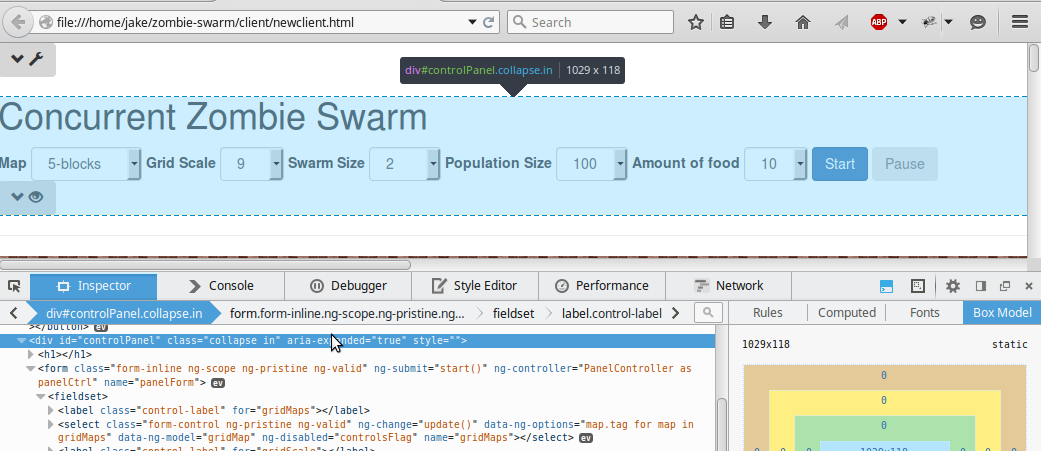
\includegraphics[width=0.7\textwidth]{img/panel.png}
\caption{System control panel}
    \label{fig:control-panel}
\end{figure}
The \verb+<body>+ element is wrapped in an JavaScript ng-controller closure, these type of closures provide scoping of JavaScript variables.
At the very top of the document a collapsible form provides access to user definable parameters of the system. Angular provides two-way data binding between HTML elements and JavaScript variables defined within the controller scope, each element of the form is bound to a corresponding variable.
A JSON object \footnote{The setup JSON is structured \{Type,Arrity,SwarmSize,PopSize,Obstructions,FoodAmount\} Using this information the \emph{environment} module can set up the simulation framework } with the values of these variables is sent over the WebSocket to set up the system. A number of predefined obstruction maps are selectable, the number of tiles in the grid is determined by the map selected. There is also a button to pause the simulation when running and a start button to begin the report loop and start the simulation.
\subsection{Angular.js}
The client software underwent one major revision, the initial version was constructed piece-by-piece in JavaScript in response to each change in the simulation architecture resulting in a lot of messy and difficult to maintain code, once the architecture was largely implemented the client was entirely rewritten using the AngularJS framework. The re-factoring into the AnuglarJS framework granted an opportunity for the convoluted logic to abstracted into a more easily maintainable code-base. The {\tt{app.js}}
source code file contains all the logic which maps variables to HTML elements and communicates with the swarm application essentially providing an control layer between the JSON data coming from the swarm application and mapping the data to the visualisation library.
\subsection{D3.js library}
\begin{figure}[h]
  \centering
  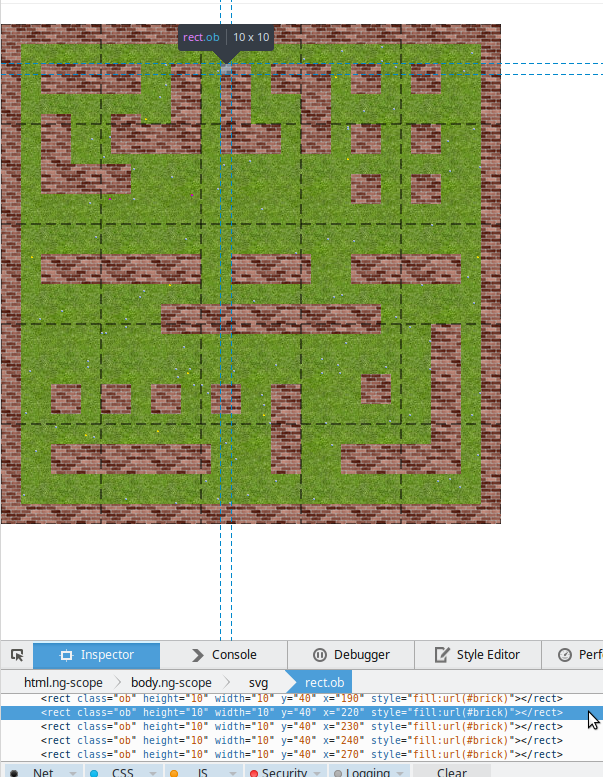
\includegraphics[width=0.7\textwidth]{img/svg-element.png}
\caption{This typical SVG visualisation contains around 3000 unique elements, without sight-lines}
    \label{fig:visualisation}
\end{figure}
In the early stages of our background research the D3 data visualisation library was identified as our visualisation solution. D3 provides a library for mapping data to elements of a scalable vector graphic image. All of the functions related to the visualisation and animation are contained in the \verb+draw.js+ source file. As the client provides important diagnostic information, almost everything visualised is from data returned over the WebSocket the only exception being the axis lines marking tile separation. All obstructions, entities and sight-lines are drawn from application data.
D3 itself provides a sophisticated model for joining data to SVG elements, updating elements based on changes in the data and removing elements form the visualisation when they are removed from the joined data.
\subsection{System pause}
We also included a button to pause the currently running simulation. Because every entity must be sent a pause signal individually you can occasionally observe slight a slight delay between one entity entering its paused state and another, it's a staggered pause rather than a hard pause. While the system is paused there is still a continuous stream of reports coming over the WebSocket the data in each report however is unchanging while the system is paused.
\subsection{Inspection panel}
\begin{figure}[h]
  \centering
  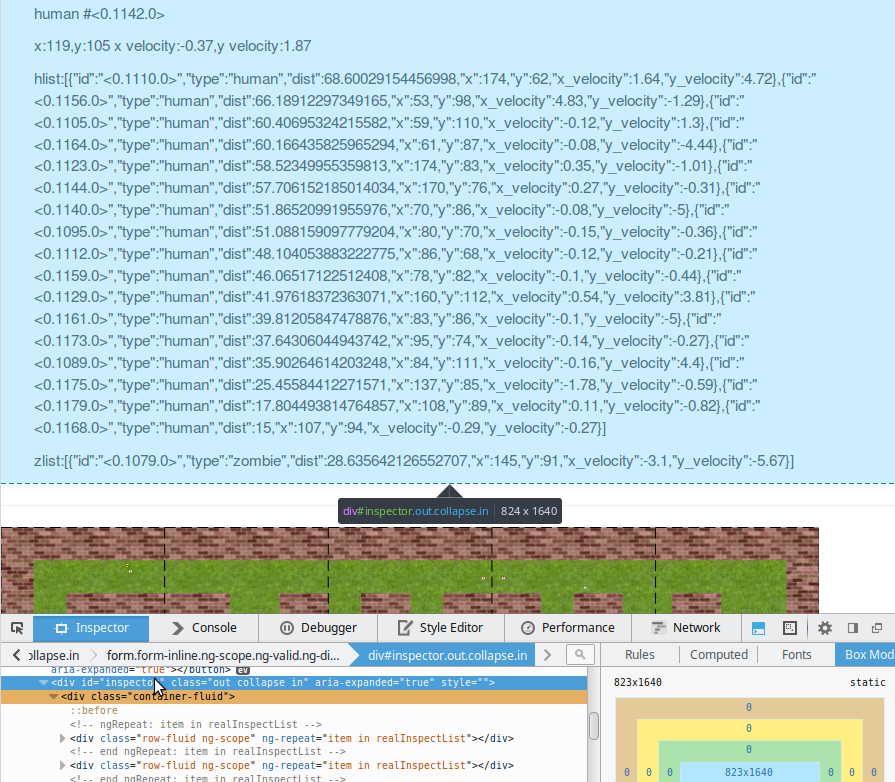
\includegraphics[width=0.8\textwidth]{img/inspector.png}
\caption{The inspector panel reveals the state of selected entities}
    \label{fig:inspector}
\end{figure}
The inspector provides continualy updated inspection of the state of selected processes, we took time to ensure that everything in the entity state is reported over the WebSocket so any aspect of an entities sate can simply be added to the inspector display. To add an entity to the inspector simply click on it in the visualisation. For detail on the implementation of the panel see section:\ref{inspector_panel}
\subsection{Sight-lines}
\label{sight_lines}
Sight lines were a late addition to the visualisation, mapping a line from each selected entity to all other entities recorded in its state, this turned out to be one of the most useful features in understanding entity state and concurrent behaviour in the simulation. More detail on sight-lines is included in Section:\ref{line_of_sight}

\subsection{Report loop}
The central function which handles communication over the WebSocket utilises a callback to pass a report request over the WebSocket at a fixed interval \footnote{We experimented with different values for the time out, there is a fine balance between state-machine time out, simulation size and WebSocket timing} when the WebSocket replies with the system data the data is passed over to the update functions in the \verb+draw.js+ module. The report loop also handles the processing of the entities selected for inclusion in the inspector.
\clearpage
\endinput
